\chapter{Software Packages}
\label{chapter:appsoft}
\thispagestyle{myheadings}

\graphicspath{{Appendix/Figures/}}


This appendix covers software architecture of two software packages that have been created during the course of the research for this thesis. The first package called Simulation for Incoherent Scatter Radar (SimISR), can create synthetic ISR data at the level of complex voltages sampled at the antenna. The other major package is called GeoData and is an advanced programing interface (API) that allows researchers to quickly import new sensor and information sources. Included are a number of functions to register, interpolate, plot and analyze this data.

\section{ISRSpectrum}
The ISR spectrum code base was developed to create the backscatter spectra from the ionosphere given a set of plasma state parameters. The code is based off of the the theoretical in \citet{kudeki:milla:1}, which has been discussed in Appendix \ref{appendix1} along with added formulations for multiple ion species.

The software is built using a simple class set up where first the user initializes an object called \textit{ISRSpectrum} using the parameters for the ISR system. After the initial definition a spectrum can be created with the method \textit{getspecsep}, which takes information on the ion species, temperatures, densities. There are optional inputs for magnetic field aspect angle, ion velocities and neutral species to calculate collision frequencies using the methods found in \citet{schunk2004ionospheres}.

\section{SimISR}

SimISR was developed to make synthetic data that one could use to create different processing algorithms and methods while having a known input or "truth" data. This simulator will take plasma fields of plasma parameters, create complex voltages from these parameters and then process that data to the point where it can estimate the input plasma parameters.

The need to create a full 3-dimensional software package was necessitated by the desire to explore the utility of the new phased array radar systems and their ability to measure 3-D fields of plasma parameters. This desire to understand the measurement capabilities of electronically scanned ISR lead to the following publication, \citet{RDS:RDS20236} where this software package was used to create reconstructions of 3-D fields of plasma parameters.

The software itself has been developed in such a way that the code mirrors the processing. An object oriented paradigm is used and thus this different processes in the processing chain are broken up in to different classes, which are: 

\begin{itemize} 
\item IonoContainer - A container class that holds information on the ionosphere or auto correlation functions (ACFs)/spectrums, both intrinsic and estimated.

\item RadarDataFile - A class that holds and operates on the radar data to create estimates of the autocorrelation function. The class takes files containing ISR spectrums and then creates ISR data and as a final step outputs instances of the IonoContainer class that holds estimates of the plasma ACF.

\item FitterMethodsGen - A class that applies the fitter to the data and outputs an instance of IonoContainer with the measured parameters. 
\end{itemize}

The overall flow can be seen in Figure \ref{fig:swflow}, where  $\Theta$ is the plasma parameters $ g(\Theta)$ is a function that turns the plasma parameters to ISR spectrums, $ \mathbf{r}$ is the spectrums/ACFs for each point of time and space, $ \mathbf{Lr}$ is the radar's operator on the spectrums/ACFs, $ \rho$ is the measured ACFs from the radar and lastly $ \hat{\Theta}$ is the estimates of plasma parameters from $ \rho$ after least squares fitting.

\begin{figure}[h!]
\centering
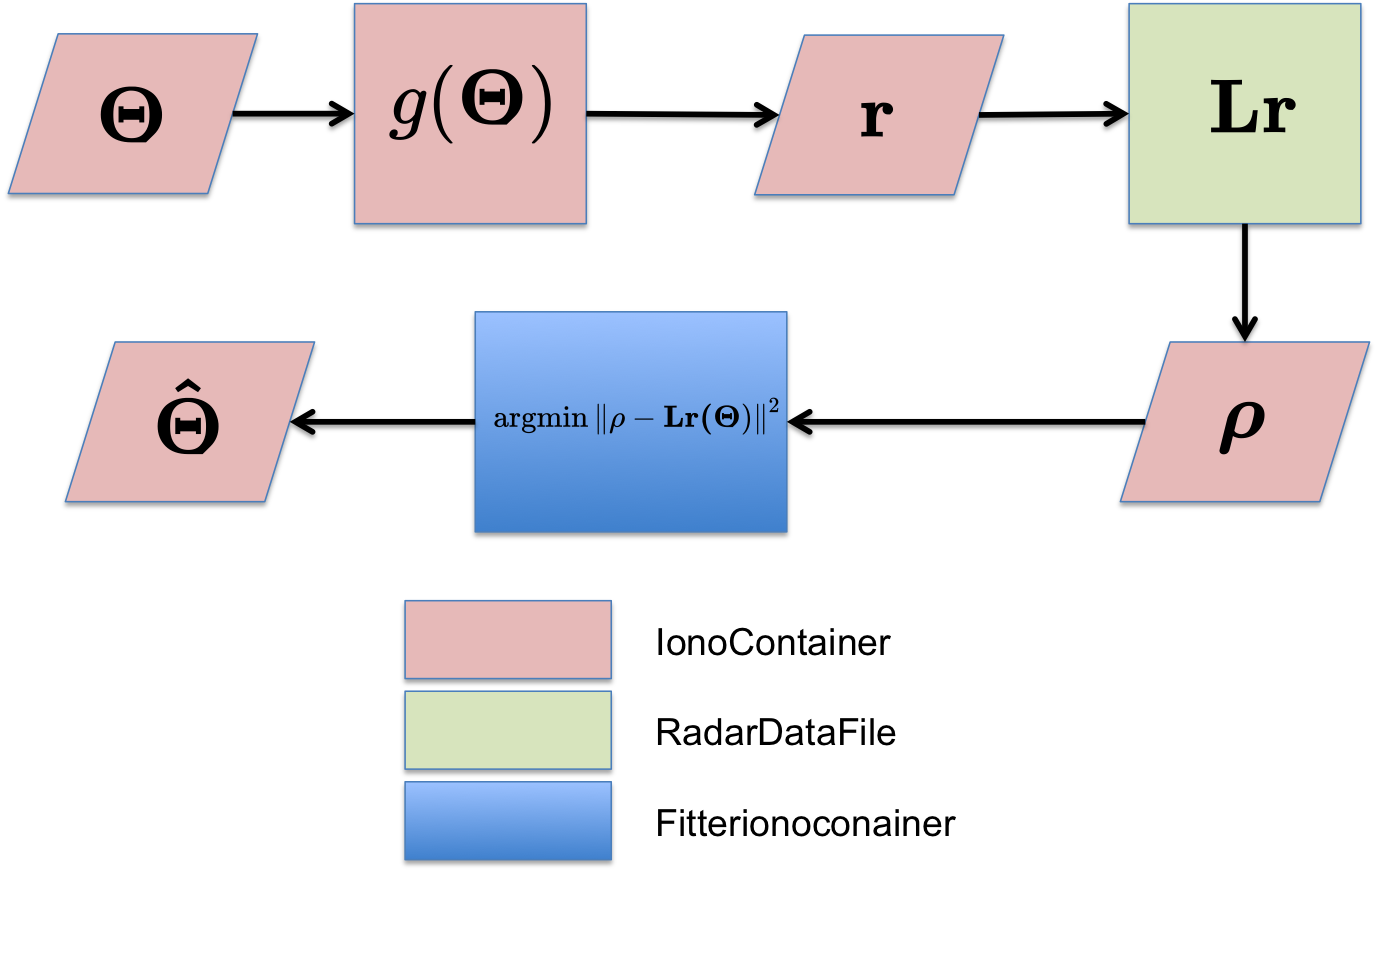
\includegraphics[width=5.0in]{softwareflowandmath}
\caption{Software flow diagram for SimISR}
\label{fig:swflow}
\end{figure}


%This report is broken up in to the following chapters. The next chapter will cover the method to calculate the ISR spectrum. There are a number of publications on this including \citep{dougherty:farley1960,hagfors1971,sheffield2010} that cover this area but we focus on the treatment found in \citep{kudeki:milla:1}. Next the method to form the ISR data will be shown, this will include the signal processing steps taken to create the data. The processing of the data from estimating the lags to fitting the plasma parameters will then be covered. We will focus on methods for long pulse but we will show where this differentiates when using other waveforms such as alternating codes and Barker codes. Lastly we will show examples of the output of the ISR simulator at a number of different spots in the processing chain.

\section{GeoData}

The GeoData project allows researchers to quickly bring in new sets of data from different sources and analyze it. The API, available both in Python and MATLAB, does this by abstracting the data set into a formatted object which can be manipulated using methods and function that are already included, thus reducing the amount of software that needs to be written. The basic object structure is shown in Figure \ref{fig:objdiag}.

\begin{figure}[h!]
\centering
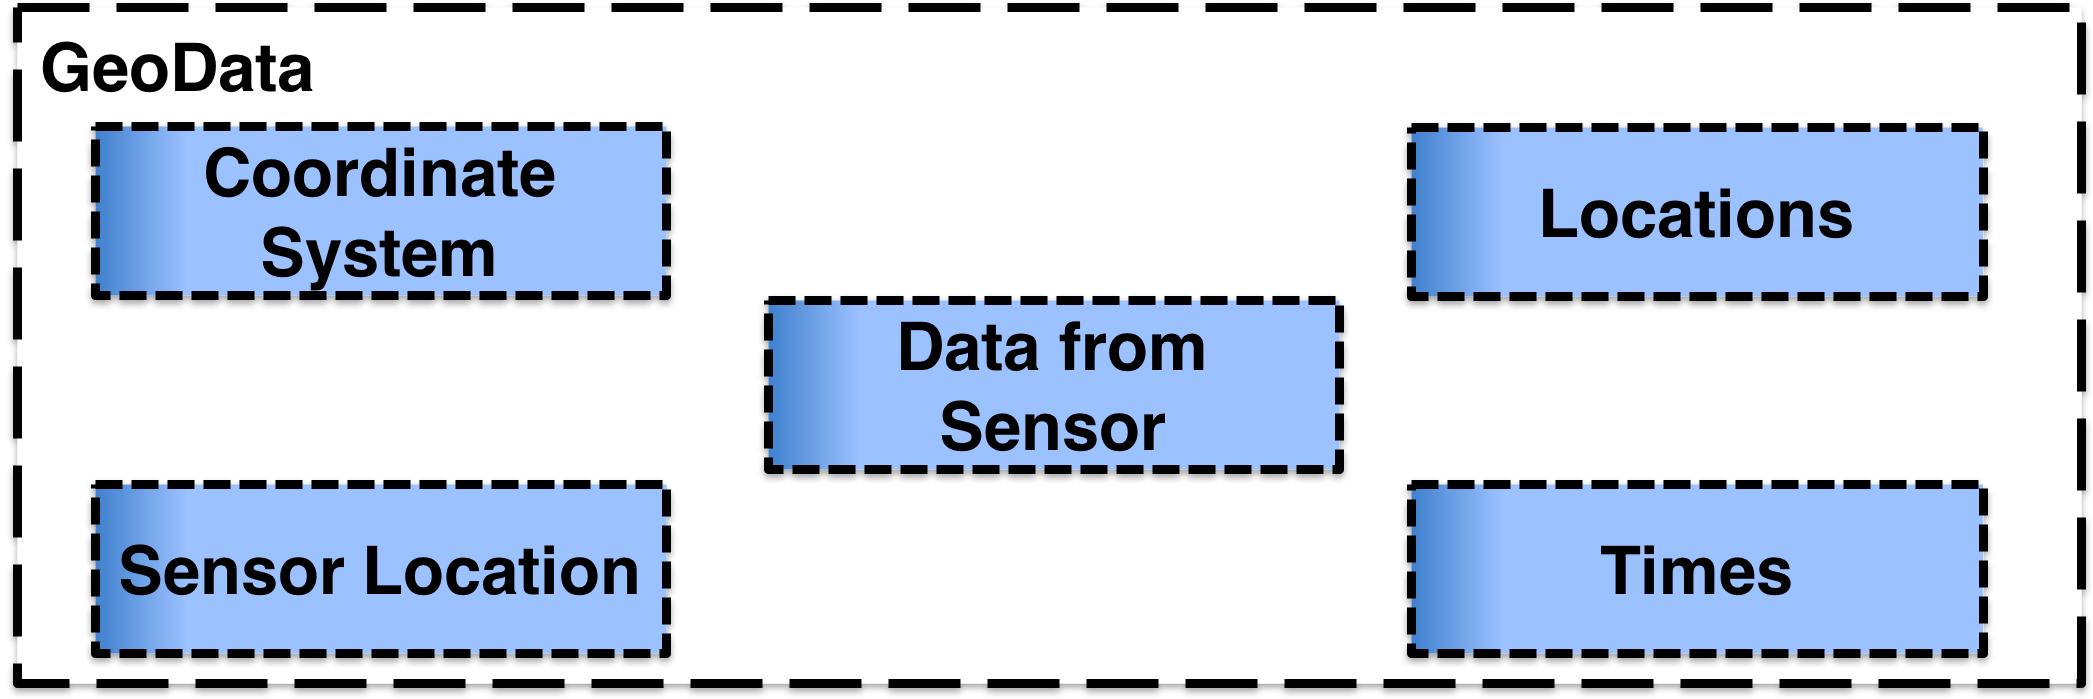
\includegraphics[width=6.0in]{geodatadiagram}
\caption{The makeup of a GeoData object.}
\label{fig:objdiag}
\end{figure}

The primary variables in a GeoData object are as follows: 
\begin{itemize} 
\item Data from Sensor - This will hold the data for the data set. In python this will be a dictionary where the keys are the names of the data and the values will be numpy arrays that hold the data. In MATLAB the field names will be the data names and the arrays will be the values. Each data set will be held in a flattened array structure or can be an NxT array where N is the number of locations of measurements and T will be the number of times.
\item Coordinate System - This string will hold the types of coordinates for the data. There will be a set number of coordinate types seen in the table below. More can be added as needed,
\item Locations - This will be a NxP array of locations in the coordinate system of choice. P is the number of elements
\item Sensor Location - This will be an array that holds the location of the sensor in wgs84. If there are multiple sensors such as a set of satellite measurements the array will be filled with nans.
\item Tims - A Tx2 array of times in posix format showing the ending and beginning of a measurement.
\end{itemize}

There are also a number of available coordinate systems that can be used as well. Table \ref{tab:coord} gives the name that it is referred to in the code base and a quick description of the system and units.

\begin{table}[]
\centering
\caption{Description of Coordinate Systems.}
\label{tab:coord}
\begin{tabular}{p{1in}p{4in}}
Name       & Description                                                                            \\
wgs84      & Latitude Longitude Altitude (deg,deg,m).                                                \\
Spherical  & Range azimuth and elevation (km, deg, deg) elevation angle is referenced to z=0 plane.  \\
Spherical2 & Range azimuth and elevation (km, deg, deg) elevation angle is referenced to x=y=0 line. \\
ENU        & East north up (m,m,m). sensorloc holds the origin.                                      \\
ECEF       & Earth centered earth fixed (m,m,m).                                                     \\
Cartesian  & Local Cartesian grid (km,km,km). Same as ENU but in km.                
\end{tabular}
\end{table}

The workflow for this package is as follows:
\begin{itemize}
\item Read In Data - The user creates a function that will read the data file into the specific variables for GeoData. Many are already available to the user for common formats.
\item Registration - If using multiple data sets overlap times must be determined. A method named \textit{timeregister} is available to do this automatically.
\item Spatial Registration - This step includes interpolating the data sets into common coordinate systems to allow for plotting.
\item Plotting - There are a number of different plotting tools available including 1-D, 2-D and 3-D plotting methods. These methods are dependent on the coordinate systems that the data are in.
\end{itemize}
